\documentclass[10pt]{beamer}

\usepackage{appendixnumberbeamer}
\usepackage{booktabs}
\usepackage[scale=2]{ccicons}
\usepackage{pgfplots}
\usepackage{graphics}
\usepackage{braket}

\usepgfplotslibrary{dateplot}
\pdfstringdefDisableCommands{\def\translate#1{#1}}
\geometry{paperwidth=140mm, paperheight=105mm}
\usetheme{metropolis}
\bibliographystyle{abbrv}
\setbeamertemplate{frame footer}{ME738 - Special Topics in Materials}

\renewcommand{\footnotesize}{\fontsize{7pt}{8pt}\selectfont}

\title{Chip Scale Atomic Clocks Sources}
\subtitle{Technology comparison}
\date{March 27, 2024}
\author{Tommaso Bocchietti}
\institute{University of Waterloo}
\titlegraphic{\hfill
\includegraphics[height=1.5cm]{pdf/UniversityOfWaterloo_logo_horiz_pms.pdf}}

\begin{document}

\maketitle

\begin{frame}{Agenda}
    \setbeamertemplate{section in toc}[sections numbered]
    \tableofcontents[hideallsubsections]
\end{frame}

\begin{frame}{Recap from "Working principles"}

    General idea: leverage the intrinsic stability of atomic transitions to discipline an oscillating circuit based on a vibrating quartz crystal.

    \begin{figure}
        \centering
        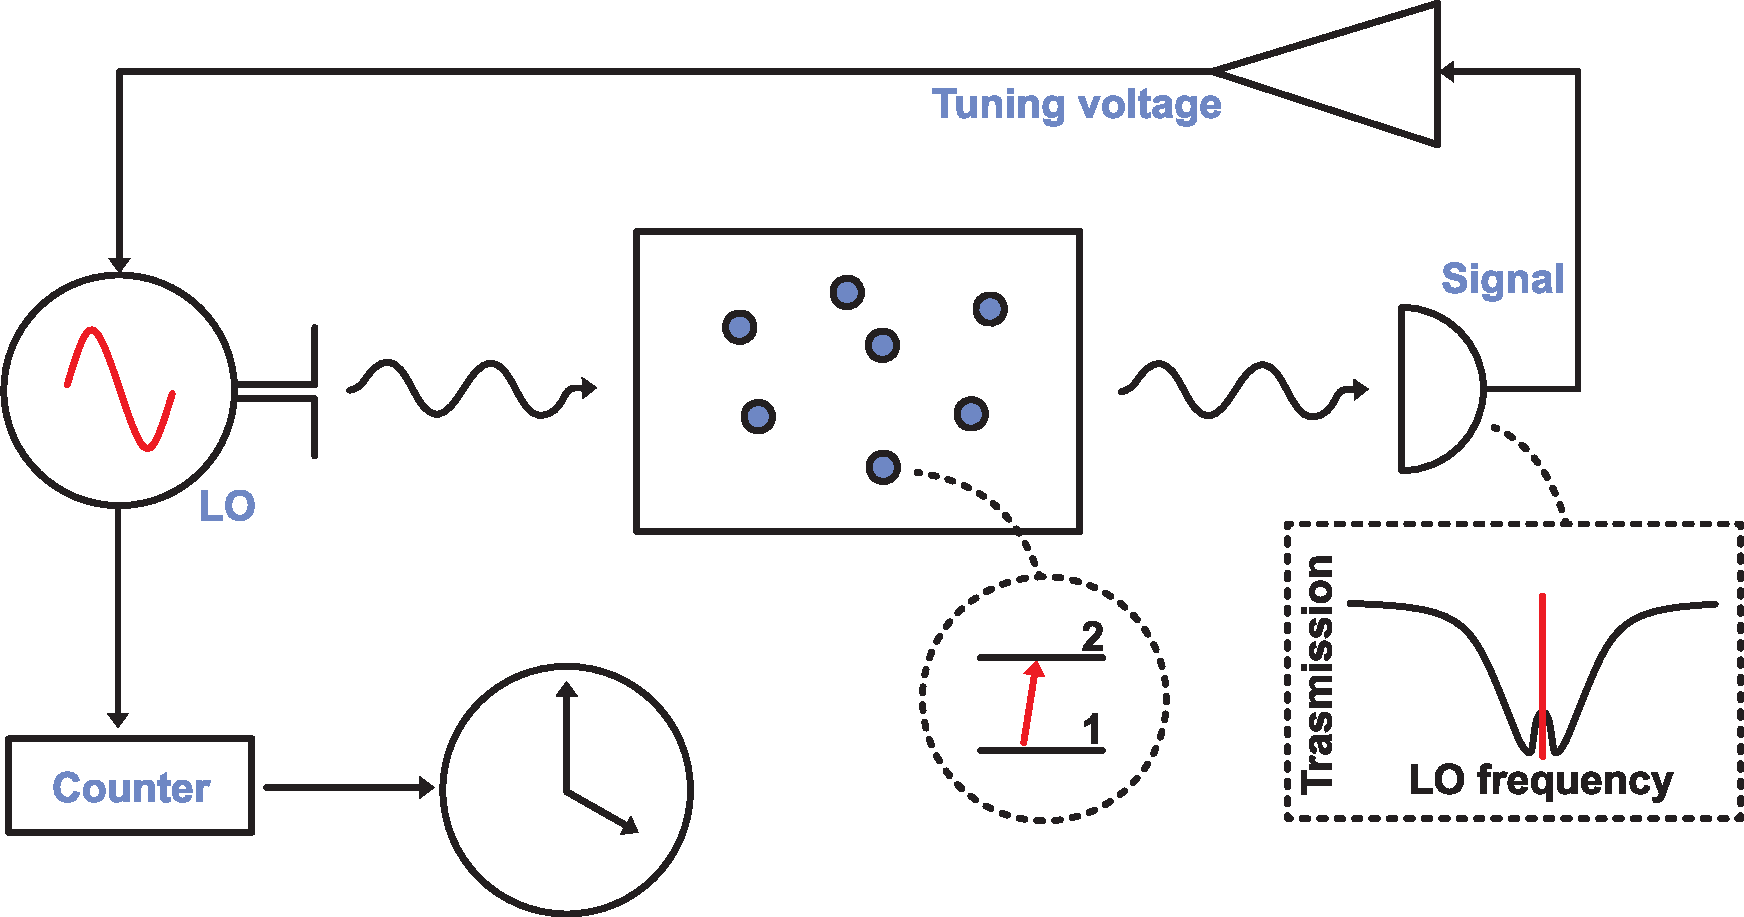
\includegraphics[width=0.9\textwidth]{pdf/CSAC-scheme.pdf}
        \caption{Chip Scale Atomic Clock scheme.}
    \end{figure}

\end{frame}

\section{Key Parameters}

\begin{frame}{Stability and Accuracy}

    \textit{
        The second, symbol $s$, is the SI unit of time.
        It is defined by taking the fixed numerical value of the $Cs$ frequency $\Delta \nu_{Cs}$, the unperturbed ground-state hyperfine transition frequency of the $^{133}Cs$ atom, to be $9.192.631.770$ when expressed in the unit $Hz$, which is equal to $s^{-1}$.
    }

    \begin{figure}
        \centering
        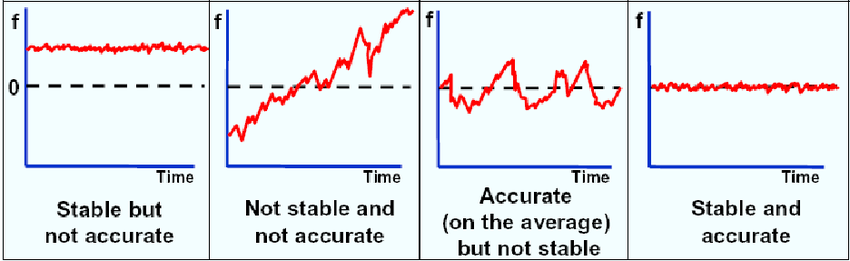
\includegraphics[width=0.9\textwidth]{img/stability-accuracy.png}
        % \caption{Accuracy and stability of an atomic clock.}
    \end{figure}

\end{frame}



\begin{frame}{Short term stability (Allan deviation $\sigma_y(\tau)$)}

    \begin{columns}[c, onlytextwidth]

        \begin{column}{0.5\textwidth}

            Allan deviation is a measure of the stability of a frequency standard.

            \begin{equation*}
                y(t) = \frac{f(t) - f_0}{f_0}
            \end{equation*}

            \begin{equation*}
                \sigma_y(\tau) = \sqrt{\frac{1}{2M} \sum_{i=2}^{M} (\bar{y}(\tau)_{i} - \bar{y}(\tau)_{i-1})^2}
            \end{equation*}

        \end{column}

        \hfill

        \begin{column}{0.45\textwidth}

            \begin{figure}
                \centering
                \only<1>{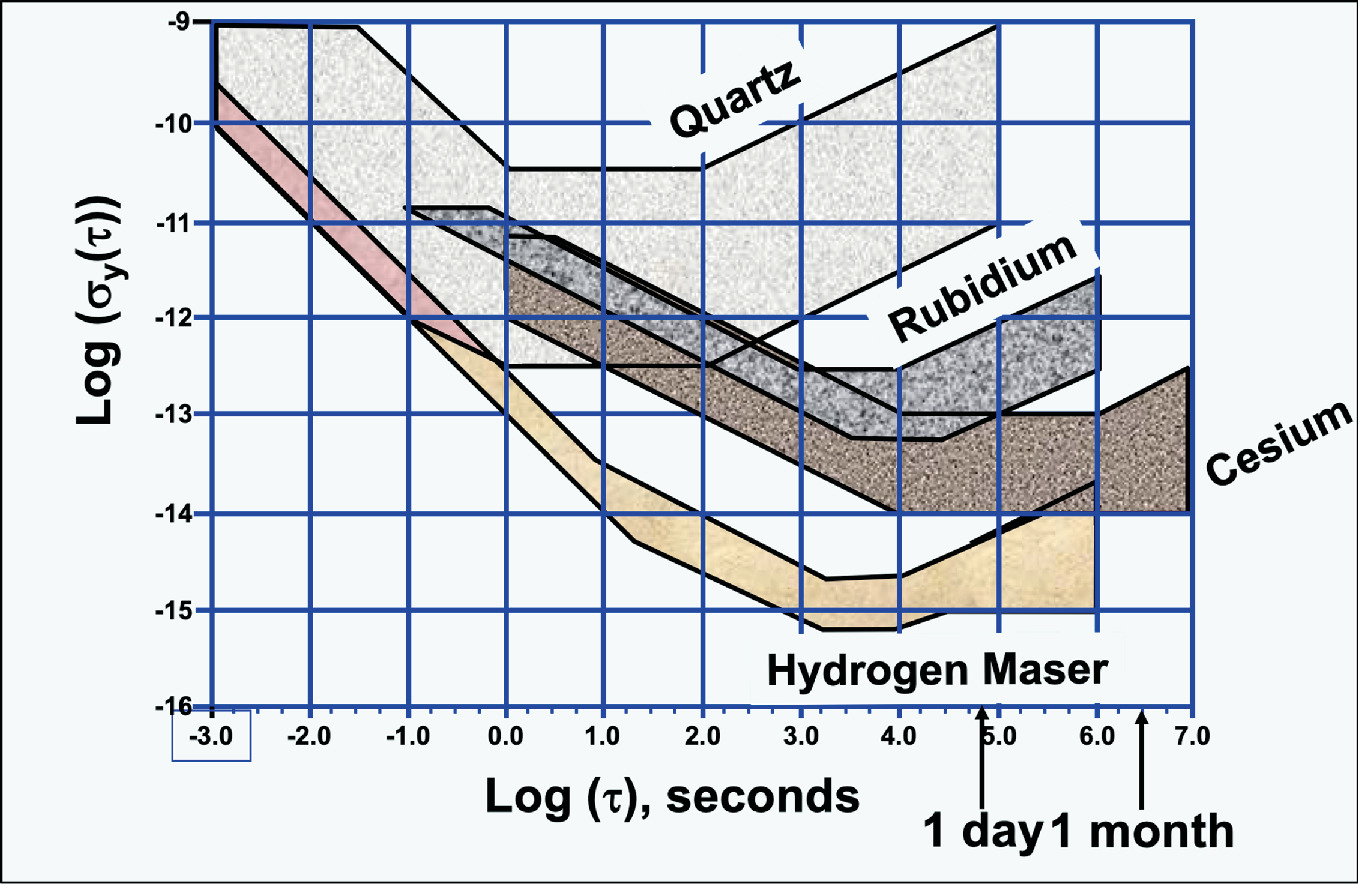
\includegraphics[width=\textwidth]{img/allan-with-quartz.png}}
                \only<2->{
                    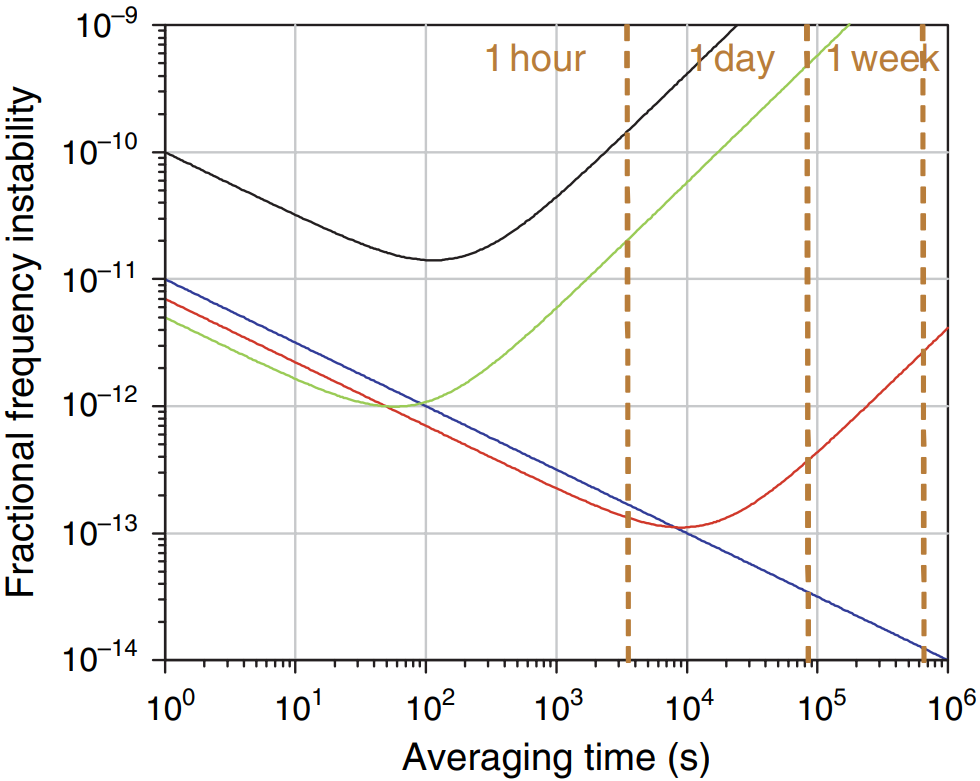
\includegraphics[width=\textwidth]{img/allan-without-quartz-2.png}
                    \caption{
                        \textcolor[HTML]{0000FF}{CBT},
                        \textcolor[HTML]{FF0000}{Rb},
                        \textcolor[HTML]{00FF00}{OCXO},
                        \textcolor[HTML]{000000}{TCXO}
                    }
                }
            \end{figure}

        \end{column}

    \end{columns}

    \only<1>{\vspace{10pt}}

    It captures the frequency \textbf{Fast Noise (mainly caused by the Local Oscillator (LO))} \& the Slow Drift (next slide)

    \footnotetext{
        $\sigma_y(\tau = 1s) = 3\times10^{-9}$ is equivalent to an instability in frequency between two observations 1 second apart with a (RMS) value of $3\times10^{-9}$.
        For a $10 MHz$ clock, this would be equivalent to $30 mHz$ RMS movement.
    }

\end{frame}



\begin{frame}{Medium term stability (Allan deviation $\sigma_y(\tau)$)}

    After the flicker floor, the \textbf{Slow Drift} became the dominant noise source and Allan deviation can be expressed as:

    \begin{equation}
        \sigma_y(\tau) = \frac{1}{Q\times SNR} \tau^{-1/2} \text{, where }
        \begin{cases}
            Q   \text{ Line quality}          & = \frac{\nu_0}{\Delta \nu}     \\
            SNR \text{ Signal-to-noise ratio} & = \frac{P_{signal}}{P_{noise}}
        \end{cases}
    \end{equation}

    \begin{columns}[c, onlytextwidth]

        \begin{column}{0.5\textwidth}

            \begin{figure}
                \centering
                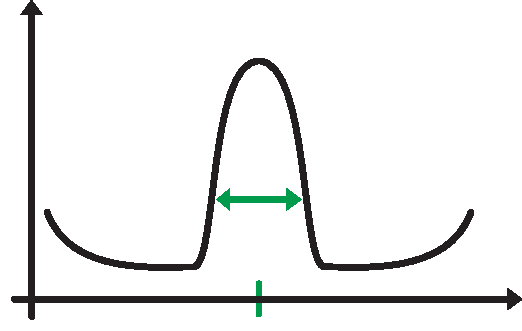
\includegraphics[width=0.7\textwidth]{pdf/Q-factor.pdf}
                \caption{$\nu_0$ and $\Delta \nu$.}
            \end{figure}

        \end{column}

        \begin{column}{0.5\textwidth}

            \begin{figure}
                \centering
                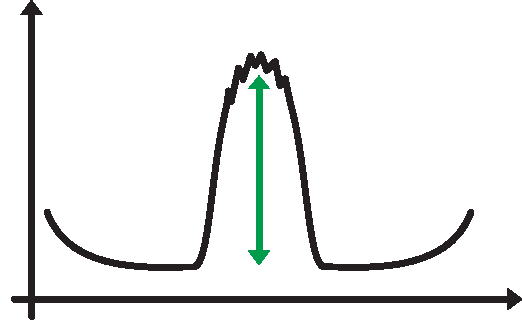
\includegraphics[width=0.7\textwidth]{pdf/P-signal.pdf}
                \caption{$P_{signal}$ and $P_{noise}$.}
            \end{figure}

        \end{column}

    \end{columns}

    \textbf{MODR}-based: lower $Q$ but higher $SNR$.\\
    \textbf{CPT}-based: higher $Q$ but lower $SNR$.

\end{frame}



\begin{frame}{Long term stability (Drift)}

    Drift is a measure of the long term stability of the clock which is caused by variation in the atomic reference frequency due to aging and environmental factors.

    \begin{figure}
        \centering
        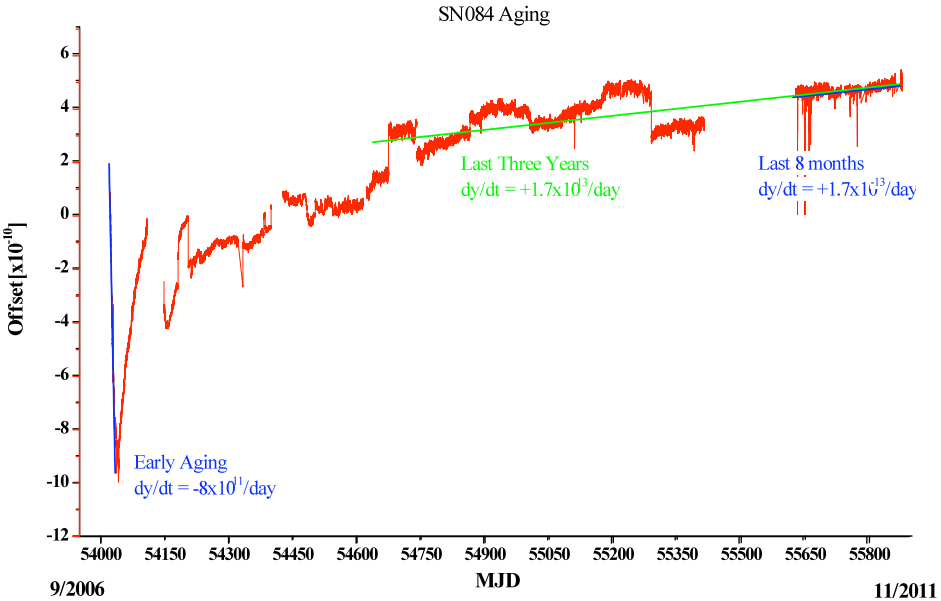
\includegraphics[width=0.7\textwidth]{img/drift.png}
        % \caption{Drift of an atomic clock.}
    \end{figure}

    % \footnotetext{Example: Drift of $10^{-10}$ means that the frequency of the oscillator changes by $10^{-10}$ per second.}
    \footnotetext{MJD: Modified Julian Dates, are a count of days since November 17, 1858.}

\end{frame}


% \begin{frame}{Thermal stability}

% \end{frame}
\section{Technology comparison}

\begin{frame}{ADEV@1s vs. Size}

    Empirical correlation\footnotemark[1]: $\sigma_y(\tau=1) = 6.85 \times 10^{-10} + \text{volume}^{-0.64}$

    \begin{columns}[c, onlytextwidth]

        \begin{column}{0.7\textwidth}

            \begin{figure}
                \centering
                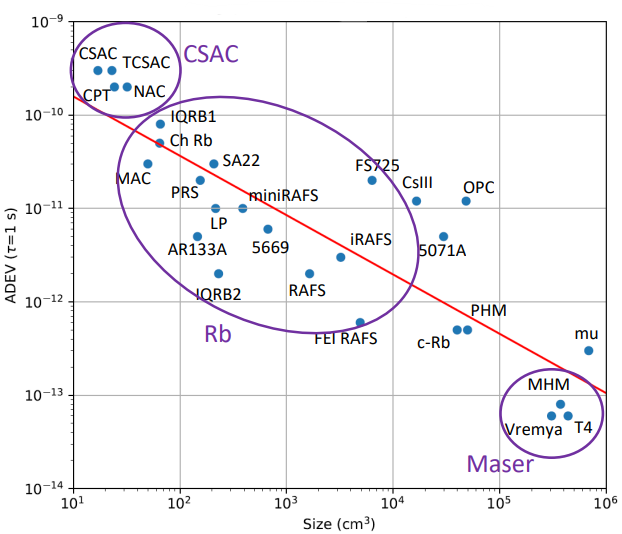
\includegraphics[width=0.9\textwidth]{img/ADEV-vs-Size.png}
                % \caption{Accuracy and stability of an atomic clock.}
            \end{figure}

        \end{column}

        \begin{column}{0.3\textwidth}

            \begin{figure}
                \centering
                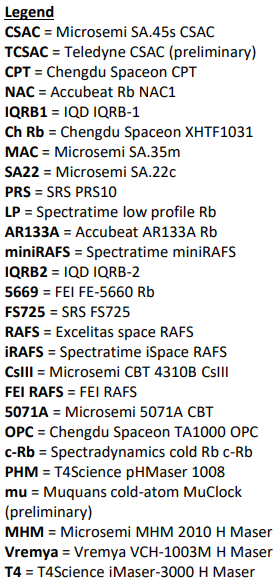
\includegraphics[width=0.83\textwidth]{img/legend.png}
            \end{figure}

        \end{column}

    \end{columns}

    \footnotetext[1]{Volume is expressed in [$cm^3$].}

\end{frame}



\begin{frame}{ADEV@1s vs. SWaP (Size, Weight and Power)}

    Similar correlation as before\footnotemark[1]: $\sigma_y(\tau=1) = 1.15 \times 10^{-10} + \text{SWaP}^{-0.27}$

    \begin{columns}[c, onlytextwidth]

        \begin{column}{0.7\textwidth}

            \begin{figure}
                \centering
                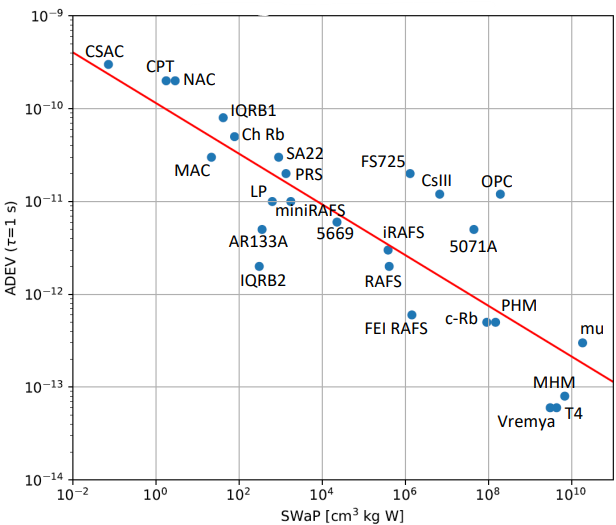
\includegraphics[width=0.9\textwidth]{img/ADEV-vs-SWaP.png}
                % \caption{Accuracy and stability of an atomic clock.}
            \end{figure}

        \end{column}

        \begin{column}{0.3\textwidth}

            \begin{figure}
                \centering
                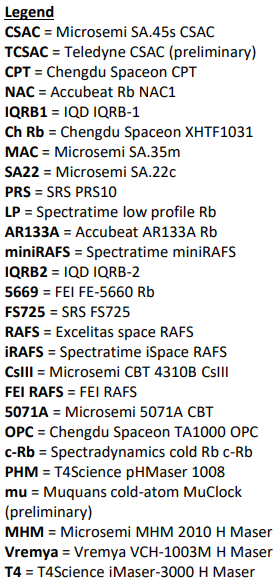
\includegraphics[width=0.83\textwidth]{img/legend.png}
            \end{figure}

        \end{column}

    \end{columns}

    \footnotetext[1]{SWaP is expressed in [$cm^3 \times kg \times W$].}

\end{frame}



\begin{frame}{Cost vs. Performance (qualitative)}

    Similar to what we have seen before, the cost of an atomic clock is proportional to its performance.

    \begin{table}
        \centering
        \resizebox{\textwidth}{!}{
            \begin{tabular}{l|llll}
                \hline
                \textbf{Technology} & \textbf{Units/year} & \textbf{Unit price} & \textbf{Worldwide sales} & \textbf{ADEV}  \\
                ~                   & ~                   & (Range in \$)       & (\$/year)                & (1 s)          \\
                \hline
                Quartz crystals     & $5 \times 10^9$     & $[0.1; 2000]$       & $5B$                     & Low to medium  \\
                CSACs               & $12000$             & $[2000; 6000]$      & $15M$                    & Medium to high \\
                Rubidium cells      & $30000$             & $[1000; 10000]$     & $150M$                   & High           \\
                Caesium beam        & $500$               & $[40000; 100000]$   & $40M$                    & Very high      \\
                Hydrogen masers     & $20$                & $>100000$           & $4M$                     & The best       \\
                \hline
            \end{tabular}
        }
        \caption{All data must be taken as indicative.}
    \end{table}

    For a CSAC, the cost is mainly driven by the packaging and assembly of the physics package.

\end{frame}

















\section{Conclusion}

\begin{frame}{Current research status for NG-CSACs}

    Despite more than 15 years since the launch of the first program to develop the NG-CSACs, many challenges remain to be addressed.

    \vspace{10pt}

    \textbf{Three possible technological solution have been proposed, but a clear winner hasn't emerged yet.}

\end{frame}



\begin{frame}{Potential and Importance of NG-CSACs}

    In conclusion, we believe that pursuing the development goals set for NG-CSACs is extremely important.

    \vspace{10pt}

    These devices will not only provide superior timing and synchronization, but they also hold the \textbf{potential to bring revolutionary technological advances in different areas} like micro and nano fabrication, quantum computing, or the understanding of fundamental physics phenomena.

\end{frame}

\appendix

\begin{frame}[standout]
    Extra slides
\end{frame}



\begin{frame}{Commercial CSACs}

    \begin{table}
        \centering
        \resizebox{!}{0.4\textheight}{
            \begin{tabular}{l|llll}
                \hline
                \textbf{Manufacturer/Model} & \textbf{Country} & \textbf{ADEV} & \textbf{Power} & \textbf{Size}           \\
                ~                           & ~                & (1 s)         & (W)            & (cm\textsuperscript{3}) \\
                \hline
                Jackson Labs CSAC GPSDO     & US               & 1E-10         & 1,4            & 85                      \\
                Seiko Epson A06860LAN       & JP               & 3E-11         & 3,0            & 75                      \\
                Precision Test Systems RFS2 & UK               & 3E-11         & 6,0            & 65                      \\
                Quartziock El O-MRX         & UK               & 5E-11         & 6,0            & 65                      \\
                Microsemi MAC SA.3Xm        & US               & 3E-11         & 5,0            & 50                      \\
                Orolia Spectratime mRO-50   & CH/FR            & 4E-11         & 0,5            & 50                      \\
                Chengdu Spaceon XHTF1031    & China            & 5E-11         & 6,0            & 50                      \\
                Microsemi MAC SA.5X         & US               & 3E-11         & 6,3            & 47                      \\
                Accubeat NAC1               & Israel           & 2E-10         & 1,2            & 32                      \\
                IQD ICPT-1                  & UK               & 9E-11         & 1,7            & 25                      \\
                Chengdu Spaceon XHTF1040    & China            & 3E-10         & 1,6            & 24                      \\
                Teledyne TCSAC              & US               & 3E-10         & 0,2            & 23                      \\
                Microsemi SA45.s            & US               & 3E-10         & 0,1            & 17                      \\
                Chengdu Spaceon XHTF1045    & China            & 3E-10         & 0,3            & 17                      \\
                \hline
            \end{tabular}
        }
    \end{table}

    \footnotetext{Data ordered by size.}

\end{frame}



\begin{frame}{Commercial atomic clocks}

    \begin{table}
        \centering
        \resizebox{\textwidth}{0.4\textheight}{
            \begin{tabular}{ll|lllllllllll}
                \hline
                \textbf{Vendor} & \textbf{Product} & \textbf{Type} & \textbf{ADEV} & \textbf{$\mathcal{L}$} & \textbf{Aging} & \textbf{Retrace} & \textbf{Tmin}          & \textbf{Tmax}          & \textbf{Tempco} & \textbf{Power} & \textbf{Weight} & \textbf{Size}           \\
                ~               & ~                & ~             & (1 s)         & (10 Hz)                & (month)        & ~                & (\textsuperscript{o}C) & (\textsuperscript{o}C) & ~               & (W)            & (kg)            & (cm\textsuperscript{3}) \\
                \hline
                Muquans         & MuC10ck          & cold Rb       & 3,00E-13      & -151                   & ~              & ~                & ~                      & ~                      & ~               & 200,00         & 135,000         & 682000                  \\
                T4Science       & iMaser-3000      & Maser         & 6,00E-14      & -136                   & 6,00E-15       & ~                & ~                      & ~                      & ~               & 100,00         & 100,000         & 436800                  \\
                Microsemi       & MHM 2020         & Maser         & 8,00E-14      & -138                   & 9,00E-15       & ~                & ~                      & ~                      & ~               & 75,00          & 246,000         & 374072                  \\
                Vremya          & VCH-1003M        & Maser         & 6,00E-14      & -135                   & 9,00E-15       & ~                & ~                      & ~                      & ~               & 100,00         & 100,000         & 305525                  \\
                T4Science       & pHMaser          & PHM           & 5,00E-13      & -130                   & 6,00E-14       & ~                & ~                      & ~                      & ~               & 90,00          & 33,000          & 49820                   \\
                Chengdu Spaceon & TA1000           & OPC           & 1,20E-11      & -125                   & ~              & ~                & ~                      & ~                      & ~               & 100,00         & 40,000          & 48266                   \\
                Spectradynamics & c-Rb             & cold Rb       & 5,00E-13      & -138                   & ~              & ~                & ~                      & ~                      & ~               & 75,00          & 30,500          & 39806                   \\
                Microsemi       & 5071A            & CBT           & 5,00E-12      & -130                   & ~              & ~                & 0                      & 55                     & ~               & 50,00          & 30,000          & 29700                   \\
                Oscilloquartz   & OSA 3235B Cs     & CBT           & 1,20E-11      & -120                   & ~              & ~                & ~                      & ~                      & ~               & 60,00          & 15,000          & 23021                   \\
                Microsemi       & cslll 4310B      & CBT           & 1,20E-11      & -130                   & ~              & ~                & 0                      & 50                     & ~               & 30,00          & 13,500          & 16544                   \\
                FEI             & FEI RAFS         & Space Rb      & 6,00E-13      & -138                   & 9,00E-13       & 5,00E-12         & -4                     & 25                     & ~               & 39,00          & 7,500           & 4902                    \\
                Spectratime     & iSpace RAFS      & Space Rb      & 3,00E-12      & -120                   & 8,30E-12       & ~                & -5                     & 10                     & ~               & 35,00          & 3,400           & 3224                    \\
                Excelitas       & RAFS             & space Rb      & 2,00E-12      & -105                   & 3,00E-12       & 5,00E-12         & -20                    & 45                     & ~               & 39,00          & 6,350           & 1645                    \\
                FEI             & FE-5669          & Rb            & 6,00E-12      & -140                   & 1,00E-11       & 2,00E-11         & -20                    & 60                     & 5,00E-11        & 20,00          & 1,690           & 669                     \\
                Microchip       & XPRO (low drift) & Rb            & 1,00E-11      & -90                    & 1,00E-11       & 3,00E-11         & -25                    & 70                     & 6,00E-10        & 13,00          & 0,500           & 455                     \\
                Spectratime     & miniRAFS         & Rb            & 1,00E-11      & -84                    & 3,00E-11       & ~                & -15                    & 55                     & ~               & 10,00          & 0,450           & 388                     \\
                IQD             & IQRB-2           & Rb            & 2,00E-12      & -138                   & 4,00E-11       & 2,00E-11         & ~                      & ~                      & ~               & 6,00           & 0,220           & 230                     \\
                Spectratime     & LP Rb            & Rb            & 1,00E-11      & -100                   & 3,00E-11       & 5,00E-11         & -25                    & 55                     & 2,00E-10        & 10,00          & 0,290           & 216                     \\
                SRS             & PRS10            & Rb            & 2,00E-11      & -130                   & 5,00E-11       & 5,00E-11         & -20                    & 65                     & 2,00E-10        & 14,40          & 0,600           & 155                     \\
                Accubeat        & AR133A           & Rb            & 5,00E-12      & -116                   & 1,00E-11       & 5,00E-11         & -20                    & 65                     & 1,00E-10        & 8,25           & 0,295           & 146                     \\
                IQD             & IQRB-1           & Rb            & 5,00E-11      & -95                    & 5,00E-11       & 2,00E-11         & 0                      & 50                     & 5,00E-10        & 6,00           & 0,105           & 66                      \\
                Chengdu Spaceon & XHTF1031 Rb      & CPT           & 5,00E-11      & -95                    & 5,00E-11       & ~                & -30                    & 65                     & 2,00E-10        & 6,00           & 0,200           & 65                      \\
                Spectratime     & mRO-50 (EAS)     & CSAC          & 4,00E-11      & -76                    & 1,50E-10       & 1,00E-10         & -10                    & 65                     & 4,00E-10        & 0,36           & 0,075           & 50                      \\
                Microsemi       & SA55 MAC         & CPT           & 3,00E-11      & -87                    & 5,00E-11       & 5,00E-11         & -10                    & 75                     & 5,00E-11        & 6,30           & 0,100           & 46                      \\
                Accubeat        & NAC              & CSAC          & 2,00E-10      & -86                    & 3,00E-10       & ~                & -20                    & 65                     & 2,00E-09        & 1,20           & 0,075           & 32                      \\
                Chengdu Spaceon & CPT              & CSAC          & 2,00E-10      & -90                    & 9,00E-10       & 5,00E-11         & -45                    & 70                     & 5,00E-10        & 1,60           & 0,045           & 24                      \\
                Teledyne        & TCSAC            & CSAC          & 3,00E-10      & -85                    & 3,00E-10       & 3,00E-10         & -10                    & 60                     & 1,00E-09        & 0,18           & 0,042           & 23                      \\
                Microsemi       & SA45.s           & CSAC          & 3,00E-10      & -70                    & 9,00E-10       & 5,00E-10         & -10                    & 70                     & 1,00E-09        & 0,12           & 0,035           & 17                      \\
                Microsemi       & SA65             & CSAC          & 3,00E-10      & -64                    & 9,00E-10       & 5,00E-10         & -40                    & 80                     & 3,00E-10        & 0,12           & 0,035           & 16                      \\
                \hline
            \end{tabular}
        }
        % \caption{Summary of current atomic frequency standard product key performance parameters}
    \end{table}

    \footnotetext{Data ordered by size.}

\end{frame}

\begin{frame}[allowframebreaks]{References}
    \nocite{*}
    \bibliography{references}
\end{frame}

\begin{frame}[standout]
    Questions?
\end{frame}

\begin{frame}[standout]
    Thank you!
\end{frame}

\end{document}